
\definecolor{purple2}{RGB}{218,112,214}

Now that enough is known about numbers, it is possible to work with non-numbers. The only known non-numbers at this point are the switches. But is knowing what they are enough to playing them? The game simpler cashing cheques will tell.

In this game there is a table with purple cheques. Each cheque has two numbers written on top, and, in each player's turn they will either pay one coin or cash a cheque that will grant him a number of coins equal to the correspondent associated integer. What is the best move for Left?

\begin{center}
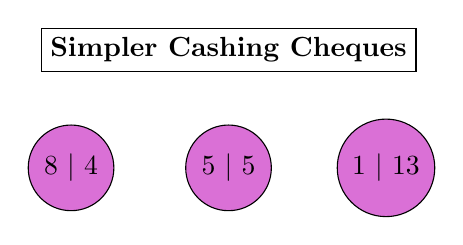
\begin{tikzpicture}
	\node[draw] (title) at (0,1.5) {\textbf{Simpler Cashing Cheques}};
	\begin{scope} [every node/.style={style=circle, draw, fill=purple2}]
		\node at (-2,0) {8 $|$ 4};
		\node at (0,0) {5 $|$ 5};
		\node at (2,0) {1 $|$ 13};
	\end{scope}
\end{tikzpicture}
\end{center}

Definitely the move is not paying, as left can earn money in his turn. A good thing to grasp from this example is that you should never play in a number, paying a coin in this case, if there are non-numbers, cashing a purple cheque in this case. Should left cash 8, 5 or 1? 1, of course. The reader is encouraged to play as left and trying to find the best possible outcome, but the answer is playing the hottest switch. Although the game above is not a switch, it is a sum of switches, and, because of that can benefit of the simplified notation discussed earlier.

\begin{align*}
	G =& (\frac{8-4}{2} \pm \frac{8+4}{2}) + (\frac{5-5}{2} \pm \frac{5+5}{2}) + (\frac{1-13}{2} \pm \frac{1+13}{2}) \\
	  =& (2 \pm 6) + (0 \pm 5) + (-6 \pm 7)\\
	  =& -4 \pm 7 \pm 6 \pm 5
\end{align*}

If you analyze the result above, it becomes clear that left must play on the rightmost component as, although it will not provide many coins, it will prevent right from cashing a huge amount. It is very possible to build scenarios where a player would even pay for cashing a cheque if that prevented the opponent from getting rich. Now that playing a simpler cashing cheques became easy, a more challenging task will rise. How to play Domineering well?

Adding a number with a temperature in a simplified position, like the expression above, should be acceptable by anyone following up to this point. Following, in the other hand, numbers will be added together with non-numbers just like number are added together and this might cause confusion. However, understanding that this sum is possible and intuitive is simple.

Playing a sum of games is just like playing a game with a set of independent rulesets and components. \begin{center}
	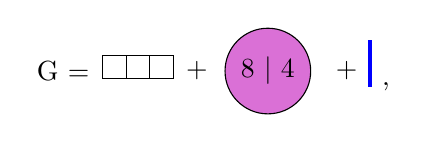
\begin{tikzpicture}
		\node at (-0.5,0.1) {G =};
		\draw[] (0,0) rectangle ++(0.3,0.3);
		\draw[] (0.3,0) rectangle ++(0.3,0.3);
		\draw[] (0.6,0) rectangle ++(0.3,0.3);
		\node at (1.2,0.1) {$+$};
		\node[style=circle, draw, fill=purple2] at (2.1,0.1) {8 $|$ 4};
		\node at (3.1,0.1) {$+$};
		\draw[color=blue, ultra thick] (3.4, -0.1) -- (3.4, 0.5);
		\node[] at(3.6, -0.1) {,};
		\end{tikzpicture}
\end{center}
for example, is a game where each player makes a move\footnote{There are other ways of playing G that will not be discussed} in any of the components and loses if cannot make a move. In other words, G is a game like every other, except for the more complex ruleset.

The result of this sum is obvious if all components are also numbers or switches. In the case of playing numbers and general non-numbers, sensible players will always play in non-numbers first. With this in mind other facts become clear. The first is that the temperature of a non-number added to a number is unaltered.

The second is that such a sum is actually a sum of non-numbers, added together with a number after they cool out. The sum of general non-numbers is thoroughly discussed in the remaining of the chapter, however, it worth noticing what the goal of this discussion is.

By the end of this section it will be thought how to convert any game in a 2D graphic composed of two \todo{curves} that collapse to one line at some point, whose axes is number x cooling factor. The purpose of all this is that if the ending point falls in the positive side, left gets an advantage, and if it falls in the positive, right does.

To build this graphic one is required to traverse the game tree, so the effort may seem fruitless as the game tree itself provides the winning strategy by itself. However, in cases where the game tree resulting from the sum of games is too large or expensive for a computer to run, there is a good strategy to playing this sum without knowing the complete game tree. In order to build the thermograph and play the \defi{thermostrat}\footnote{This text will not present the thermostrat} correctly, there are a lot of minor concepts not discussed yet.

Other than the bias, playing a game like Domineering well involves the concepts of \defi{left/right stops}, \defi{toenail}, \defi{ambient temperature}, \defi{freezing point}, \defi{cooling}, \defi{heating} and a few others. To put all that together and provide a clear visualization of the best strategy, the thermograph.

\begin{center}
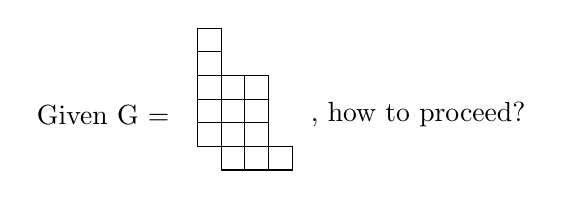
\begin{tikzpicture}
	\node at (-1.5,0.1) {Given G =};
	\draw[] (0,-0.6) rectangle ++(0.3,0.3);
	\draw[] (0.3,-0.6) rectangle ++(0.3,0.3);
	\draw[] (0.6,-0.6) rectangle ++(0.3,0.3);
	\draw[] (-0.3,-0.3) rectangle ++(0.3,0.3);
	\draw[] (0,-0.3) rectangle ++(0.3,0.3);
	\draw[] (0.3,-0.3) rectangle ++(0.3,0.3);
	\draw[] (-0.3,0) rectangle ++(0.3,0.3);
	\draw[] (0,0) rectangle ++(0.3,0.3);
	\draw[] (0.3,0) rectangle ++(0.3,0.3);
	\draw[] (-0.3,0.3) rectangle ++(0.3,0.3);
	\draw[] (0,0.3) rectangle ++(0.3,0.3);
	\draw[] (0.3,0.3) rectangle ++(0.3,0.3);
	\draw[] (-0.3,0.6) rectangle ++(0.3,0.3);
	\draw[] (-0.3,0.9) rectangle ++(0.3,0.3);
	\node at (2.5,0.1) {, how to proceed?};
\end{tikzpicture}
\end{center}

\begin{center}
	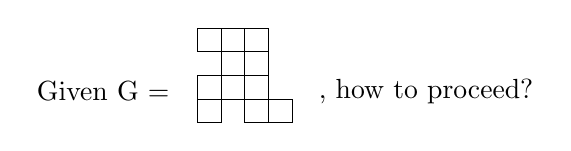
\begin{tikzpicture}
		\node at (-1.2,0.1) {Given G =};
		\draw[] (0.6,-0.3) rectangle ++(0.3,0.3);
		\draw[] (0.9,-0.3) rectangle ++(0.3,0.3);
		\draw[] (0,-0.3) rectangle ++(0.3,0.3);
		\draw[] (0,0) rectangle ++(0.3,0.3);
		\draw[] (0.3,0) rectangle ++(0.3,0.3);
		\draw[] (0.6,0) rectangle ++(0.3,0.3);
		\draw[] (0.3,0.3) rectangle ++(0.3,0.3);
		\draw[] (0.6,0.3) rectangle ++(0.3,0.3);
		\draw[] (0,0.6) rectangle ++(0.3,0.3);
		\draw[] (0.3,0.6) rectangle ++(0.3,0.3);
		\draw[] (0.6,0.6) rectangle ++(0.3,0.3);
		\node at (2.9,0.1) {, how to proceed?};
	\end{tikzpicture}
\end{center}

G is definitely not a switch nor a sum of switches. It is possible to say the temperature in G is going to stay high for quite some time, because hotness is a term used to define the importance of the next move. A good place to start is writing out the game tree and building a temperature graphic of how it builds up from simpler positions until the more complicated ones.

To decrease the confusion that builds up in complicated positions, there is the idea of a cooling factor. The non-number \Gm{} cooled by $t$ degrees is represented by \Gm{_t} and is defined by:
\begin{center}
	\Gm{_t} = \gam{\Gm{^L_t} - t}{\Gm{^R_t} + t} $\forall t \leq t'$\\
	\Gm{_t} = x $\forall t > t'$\\
	Given $t'$ is the smallest cooling factor such\\
	that \Gm{_{t'}} is infinitesimally close to a number $x$,
\end{center}

The temperature $t(G)$ is equal to $t'$. Now that both axes are defined, some examples of thermographs:

\begin{tikzpicture}
	\begin{axis}
		[
		title = \Gm{=} \gam{3}{1},
		xmin=0.5,xmax=3.5, x dir=reverse, xtick={0, 1, 2, 3},
		ymax=3, ytick={0, 0.5, 1},
		axis x line*=none, axis y line*=none,
		axis line style={draw=none},
		y label style={rotate=-90,at={(current axis.north west)}, right=5mm},
		ylabel = \textbf{t}
		]
		\addplot[black] coordinates {
		(0.5,0)(3.5,0)
		};
		\addplot[black, very thick] coordinates {
		(0.9,-0.1)(2,1)
		};
		\addplot[black, very thick] coordinates {
		(3.1,-0.1)(2,1)
		};
		\addplot[black,-{Latex[length=3mm]}, very thick] coordinates {
		(2,1)(2,2)
	};
	\end{axis}
	\begin{axis}
	[
	at={(0.5\linewidth,0)},
	title = \Gm{=} \gam{0}{{-}4},
	xmin=-4.5,xmax=0.5, x dir=reverse, xtick={-4, -2, 0},
	ymax=3, ytick={0, 1, 2},
	axis x line*=none, axis y line*=none,
	axis line style={draw=none},
	y label style={rotate=-90,at={(current axis.north west)}, right=5mm},
	ylabel = \textbf{t}
	]
	\addplot[black] coordinates {
		(0.5,0)(-4.5,0)
	};
	\addplot[black, very thick] coordinates {
		(-0.1,-0.1)(-2,2)
	};
	\addplot[black, very thick] coordinates {
		(-4.1,-0.1)(-2,2)
	};
	\addplot[black,-{Latex[length=3mm]}, very thick] coordinates {
		(-2,2)(-2,2.5)
	};
	\end{axis}
	\begin{axis}
	[
	at={(0,-330)},
	title = \Gm{=} \gam{0}{0},
	xmin=-0.5,xmax=0.5, x dir=reverse, xtick={0},
	ymax=2, ytick={0, 1},
	axis x line*=none, axis y line*=none,
	axis line style={draw=none},
	y label style={rotate=-90,at={(current axis.north west)}, right=5mm},
	ylabel = \textbf{t}
	]
	\addplot[black] coordinates {
		(-0.5,0)(0.5,0)
	};
	\addplot[black, very thick] coordinates {
		(-0.1,-0.1)(0,0)
	};
	\addplot[black, very thick] coordinates {
		(0.1,-0.1)(0,0)
	};
	\addplot[black,-{Latex[length=3mm]}, very thick] coordinates {
		(0,0)(0,1.5)
	};
	\end{axis}
	\begin{axis}
	[
	at={(0.5\linewidth,-330)},
	title = \Gm{=} \gam{0}{\gam{0}{0}},
	xmin=-0.5,xmax=0.5, x dir=reverse, xtick={0},
	ymax=2, ytick={0, 1},
	axis x line*=none, axis y line*=none,
	axis line style={draw=none},
	y label style={rotate=-90,at={(current axis.north west)}, right=5mm},
	ylabel = \textbf{t}
	]
	\addplot[black] coordinates {
		(-0.5,0)(0.5,0)
	};
	\addplot[black, very thick] coordinates {
		(0,-0.1)(0,0)
	};
	\addplot[black, very thick] coordinates {
		(0.1,-0.1)(0,0)
	};
	\addplot[black,-{Latex[length=3mm]}, very thick] coordinates {
		(0,0)(0,1.5)
	};
	\end{axis}
\end{tikzpicture}


Some characteristics might be immediately apparent. The first is that the x-axis is reversed. The reason for that is to keep Right's movements to the right and Left's to the left. The second characteristic may be that all the thermographs end with a vertical \defi{mast}. The mast begins at $t'$ and indicates that \Gm{} is a number from that point forward. The last one is that the graphic continues past the $y=0$ line. It is worth noticing that the difference between the last two thermographs is below the $y=0$ line.

Toenails, the segments below the $y=0$ line, are important, but they are actually simple extensions of the graphic. The reason for the last two toenails to be different is that cooling is applied to all the left and right alternatives, but in opposite directions. It is important to remember \Gm{_t} = \gam{\Gm{^L_t} - t}{\Gm{^R_t} + t}, because it explains the difference. Both Left's and the first Right's toenail came from cooling 0, but the second Right's toenail came from cooling \gam{0}{0}.

The next example, the first of non-switch hot games, shows how cooling $L$ and $R$ alternatives work.\\
\begin{center}
\begin{tikzpicture}
	\begin{axis}
		[
		title = \Gm{=}\gam{\gam{3}{1}}{\gam{0}{{-}4}}
		xmin=-4.5,xmax=3.5, x dir=reverse, xtick={-2, -4, -1, 0, 1, 2, 3},
		ymax=2.5, ytick={0, 0.5, 2},
		axis x line*=none, axis y line*=none,
		axis line style={draw=none},
		y label style={rotate=-90,at={(current axis.north west)}, right=5mm},
		ylabel = \textbf{t},
		scale=2
		]
		\addplot[black] coordinates {
			(-4.5,0)(3.5,0)
		};
		\addplot[black, ultra thick] coordinates {
		(0.9,-0.1)(2,1)
		};
		\addplot[black] coordinates {
			(3.1,-0.1)(2,1)
		};
		\addplot[black,-{Latex[length=3mm]}, very thick] coordinates {
			(2,1)(2,2)
		};
		\addplot[black, ultra thick] coordinates {
		(-0.1,-0.1)(-2,2)
		};
		\addplot[black] coordinates {
			(-4.1,-0.1)(-2,2)
		};
		\addplot[black,-{Latex[length=3mm]}, ultra thick] coordinates {
			(-2,2)(-2,2.5)
		};
	\end{axis}
\end{tikzpicture}
\end{center}









